In this section, we evaluate the quality of uncertainty and confidence measures proposed in~\cref{sec:methods}.


\subsection{Setup for experiments}

\textbf{Datasets}
Following \citet{kuhn2023semantic}, we use the open-book conversational question answering dataset, CoQA (\datasetcoqa)~\citep{reddy-etal-2019-coqa}, and the closed-book QA dataset, TriviaQA (\datasettrivia)~\citep{joshi-etal-2017-triviaqa}.
In addition, we also use the more challenging closed-book QA dataset, Natural Questions (\datasetnqopen)~\citep{kwiatkowski-etal-2019-natural}.
We use the development split of \datasetcoqa with 7,983 questions, the validation split of \datasetnqopen with 3,610 questions, and the validation split of the \texttt{rc.nocontext} subset of \datasettrivia with 9,960 (de-duplicated) questions. 
We repeat all experiments 10 times, each time with a random subset of 1,000 questions as the calibration set for hyper-parameters of $U$ and $C$ measures, and test the performance on the remaining data. 
We report the mean and standard deviation of all evaluation metrics (see~\cref{sec:exp:eval}). 

\textbf{LLMs}
We followed \citet{kuhn2023semantic} and include OPT~\citep{zhang2022opt} in our experiments.
We also test three more recent models that have demonstrated superior performance: LLaMA~\citep{touvron2023llama}, LLaMA2~\citep{touvron2023llama2} and the black-box \texttt{gpt-3.5-turbo} served by OpenAI via an API\footnote{All \texttt{gpt-3.5-turbo} used in this paper are the \texttt{0301} version.}.
For both LLaMA and OPT, we use the 13B versions.
We use the default generation configs for all models.

\textbf{Baselines}
We compare all uncertainty and confidence measures listed in \cref{sec:methods}, including \baselineNumSets, \methodDegree, \methodEcc and \methodEigvClip.
\methodDegree, \methodEcc and \methodEigvClip are constructed with three versions using $\affinityJaccard$, $\affinityEntail$, $\affinityContradict$ (with suffix J/E/C, respectively).
We also include ``lexical similarity'' ($U_\baselineLexiSim$) from \citet{kuhn2023semantic} which measures the average rougeL between responses.
Note that only $U_{\baselineNumSets}$ and $U_{\baselineLexiSim}$ have appeared in literature before~\citep{kuhn2023semantic}.
To benchmark these methods with the existing literature, we include two \textit{white-box} baselines for non-GPT LLMs: 
\begin{itemize}
    \item Semantic Entropy (\baselineGal)~\citep{kuhn2023semantic}:
    This uncertainty estimate ($U_{\baselineGal}$) groups answers like \baselineNumSets, and then computes the entropy over the aggregated semantic sets.
    This requires access to the token-level logits from the base LLM.
    %We present only the un-normalized version as we observed in our experiments that the normalized version is typically worse. 
    \item \baselinePTrue~\citep{kadavath2022language}:
    This confidence measure $C_{\baselinePTrue}$ estimates the probability that a model's generation is correct by asking the model itself\footnote{Note that \baselinePTrue may not require white-box access if one is willing to sample a lot of responses from the LLM, which is however computationally expensive.}.
    We follow the prompts provided in~\cite{kuhn2023semantic,kadavath2022language}, and convert $C_{\baselinePTrue}$ to an uncertainty estimate $U_{\baselinePTrue}$ by taking the average over all responses.
    
\end{itemize}


\subsection{Evaluation}\label{sec:exp:eval}

\textbf{Evaluation Metrics}: 
Effective uncertainty measures must reflect the reliability of LLM responses, with higher uncertainty and lower confidence more likely leading to incorrect generations.
Following prior works~\citep{kuhn2023semantic,Band2022BenchmarkingBD}, we evaluate the quality of the proposed UQ measures by using them to predict whether a generation is correct or not, and compute the Area Under Receiver Operating Characteristic (\textbf{AUROC}) for such prediction.
Specifically, if we denote $acc_{i,j}=\mathbbm{1}\{\mathbf{s}_{i,j} \text{ correctly answers } x_i\}$, we compute average AUROC using $C(x_\cdot, \mathbf{s}_{\cdot,j})$ to predict $acc_{\cdot, j}$ for $j\in[m]$.
Unless otherwise noted, $m=20$.

AUROC however bears two limitations: it can only be applied on binary labels, and its value is hard to interpret.
Thus, we use Area Under Accuracy-Rejection Curve (\textbf{AUARC})~\citep{auarc}, as an alternative evaluation metric\footnote{While originally AUARC was defined with a binary accuracy label, one could generalize it to any continuous label, such as the expected accuracy (using a Monte Carlo estimate).}.
Illustrated in \cref{fig:auroc_auarc}, Accuracy-Rejection Curve (ARC) is computed as the average \textit{target} (i.e. accuracy) when we reject a subset of the samples basing on \textit{predictor} (i.e. $U$ or $C$).
As we reject more high-uncertainty samples, the remaining samples should have higher accuracy.
The ``Oracle'' (max) AUARC is achieved by directly using the \textit{target} as the \textit{predictor}, while the AUARC of a random \textit{predictor} equals to the base accuracy without rejection. 


\textbf{Correctness of Generations}:
We assess the correctness of the generated responses automatically using \texttt{gpt-3.5-turbo} from the OpenAI API. This model is provided with the question, reference answer, and LLM-generated response, and it assigns a correctness score between 0 and 1. Responses with scores above 0.7 are deemed correct. 
Like~\cite{kuhn2023semantic} (which used rougeL score as a heuristic to evaluate the correctness of generated responses), we also perform human verification on the correctness of the auto-generated judgment by \texttt{gpt-3.5-turbo} and found that the accuracy is about 0.95 (see the Appendix for more details).


\begin{figure}[ht]
    \centering
    %\vspace{-3mm}%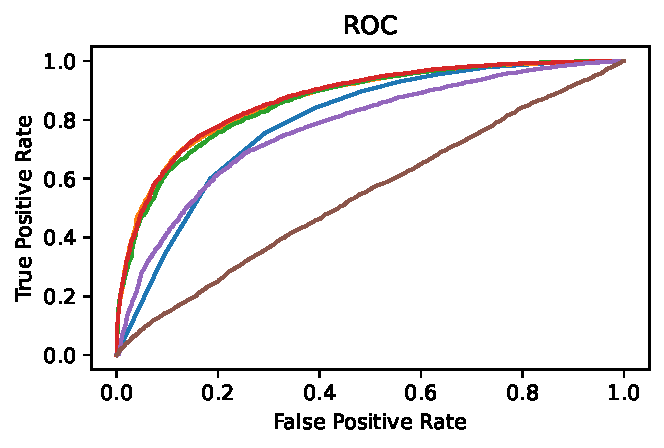
\includegraphics[width=0.45\textwidth]{pics/trivia_llama_auroc.pdf}%
    %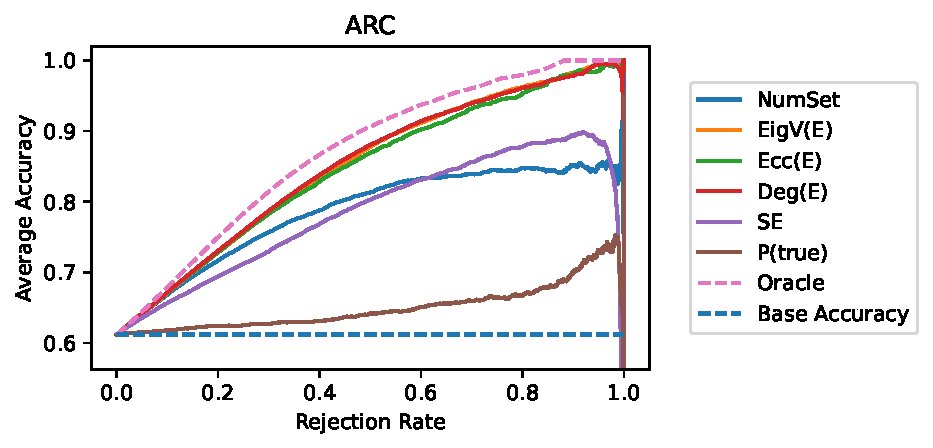
\includegraphics[width=0.45\textwidth]{pics/trivia_llama_auarc.pdf}
    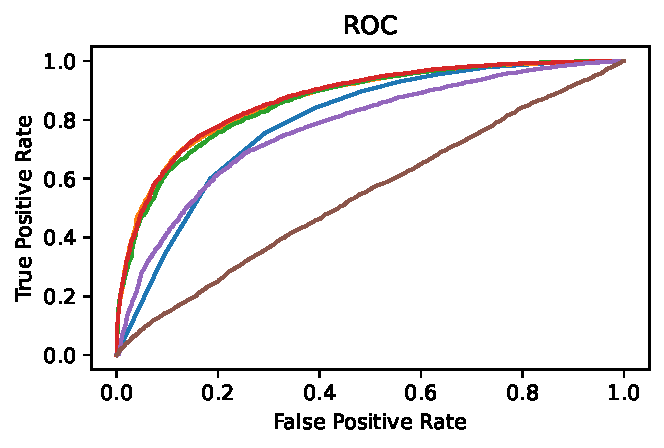
\includegraphics[height=4.5cm]{pics/trivia_llama_auroc.pdf}%
    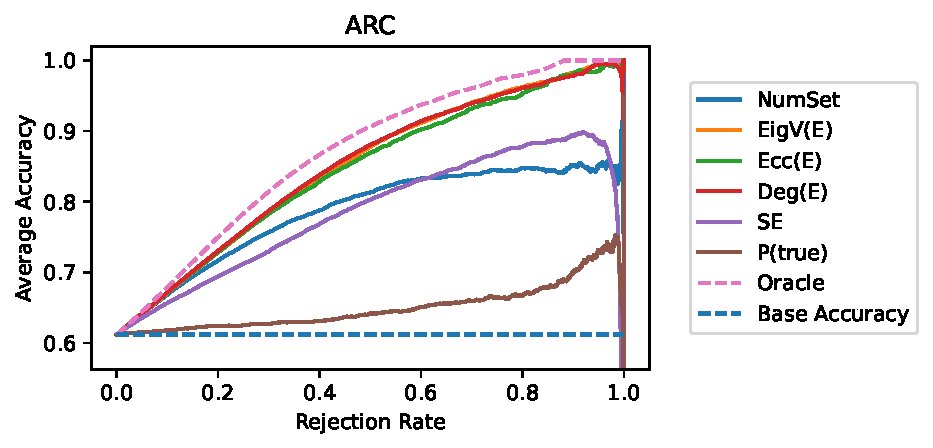
\includegraphics[height=4.5cm]{pics/trivia_llama_auarc.pdf}
    \caption{The ROC (left) computed using the accuracy of the 1st generated response and the corresponding confidence $C$ (when available, otherwise $U$), for LLaMA on \datasettrivia.
    ARC (right) is computed using $U$ and expected accuracy. 
    (For ARC, average accuracy is noisy at high rejection rate due to small sample size.) 
    The suffix (E) denotes for $a_{NLI,entail}$. %(see \cref{sec:exp:baselines} for more details).
    Different ways to construct $U$ or $C$ from $a_{NLI,entail}$ make a relatively small difference, but are all noticeably better than the baselines (including the white-box baselines).
    The ARC suggests that if we select only the top 50\% samples using, for example, \methodDegree(E), we could improve the accuracy from 62\% to around 90\%. 
    }
    \label{fig:auroc_auarc}
\end{figure}



%\subsection{Baselines}\label{sec:exp:baselines}

 



\begin{figure}[ht]
    \centering
    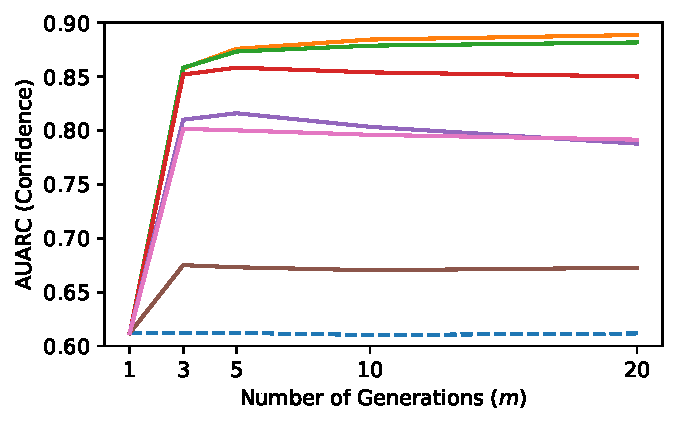
\includegraphics[height=3.2cm]{pics/trivia_llama_conf_auarc_by_numgens.pdf}%
    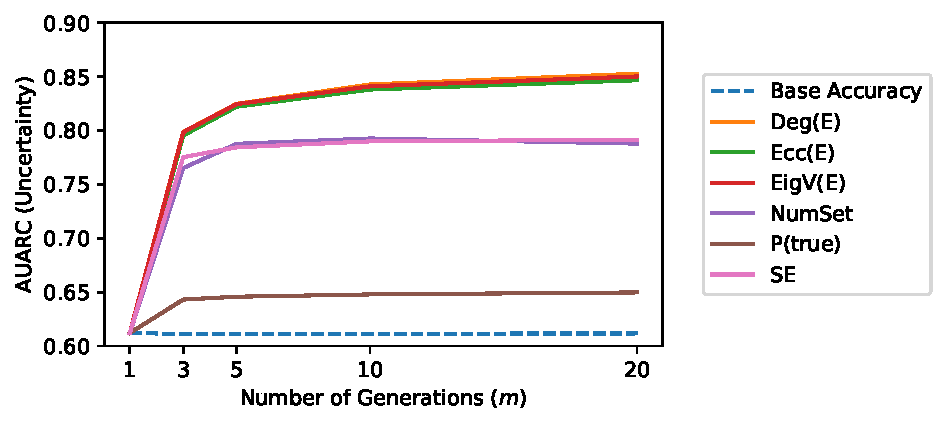
\includegraphics[height=3.2cm]{pics/trivia_llama_auarc_by_numgens.pdf}
    \caption{
    AUARC for confidence (left) and uncertainty (right), with different number of sampled responses. 
    A small $m$ like 3 already greatly improves the accuracy in selective generation, compared with no rejection or rejection based on random noise (Base Accuracy).
    In general, confidence-based measures (\methodDegree and \methodEcc) achieve better performance in the C+IA setting, confirming the intuition that response-dependent confidence measures predict the quality of individual responses better.
    %Note that the expected accuracy is always computed with 20 generations as it represents the best measurement. 
    %it happens that for this particular setup, the individual auc for the first three are high: (SE) 0.795,0.803,0.799,0.769,0.772,0.770,0.770,0.769,0.764,0.777,0.772,0.765,0.772,0.771,0.778,0.768,0.767,0.774,0.769,0.774. as a result, as we increase the number of generatiosn on the left, the aucs go down.
    }
    \label{fig:auarc_by_num_gens}
\end{figure}


\subsection{Results}\label{sec:exp:results}
%In this section, we focus on results with $m$=10, deferring additional results to the Appendix.

\begin{figure}[htb]
  \centering
  \begin{minipage}{\textwidth}
  {\small
        \begin{verbatim}
Q: why was the plague that struck athens so devastating
A: close quarters and poor hygiene

10 Generations:
There's no cure
a large flock of birds
because the plague was unknown at the time
The plague was devastating then because the diseases were unknown and a mystery to the \
    ancient world and the there where numerous diseases spread
it was so short and caused so much quaratic
Athens was located within a part of Greece that was full of fleas
The plague of Athens was a pandemic that hit the Greek city of Athens and surrounding \ 
    areas in 429-428 BC
Soldiers returning from battle
because they were
because it happened just as farming season began
        \end{verbatim}
}
  \end{minipage}
  \caption{An example where contradiction-based $U_{\methodEigvClip}$ indicates low uncertainty, % (15.4\% percentile), 
  yet the generated responses are mostly low-quality.
  Entailment-based similarity suggests high uncertainty. % at 87.9\% percentile.
  }
  \label{example:lowcontra:main}
% index=2827, llama2, nq_open
\end{figure}

\textbf{Uncertainty Measures}:
We first evaluate the uncertainty measures by using them as the predictor to predict \textit{expected accuracy} (shorthanded as U+EA), estimated with $\hat{\mathbb{E}}[acc_i] = \frac{1}{m}\sum_{j=1}^{m} acc_{i,j}$ (m=20).
The AUARCs are shown in \cref{table:main:exp:arc:u+ea} (AUROC is skipped as expected accuracy is not binary).
For readability, we include only $\affinityEntail$ which empirically performs the best, with full experiment results in the Appendix. 
We hypothesize that $\affinityEntail$ outperforms $\affinityContradict$ because even if generations do not contradict each other, they could be still mostly meaningless, whereas generations that actually align could indicate low uncertainty.
A such example could be found in \cref{example:lowcontra:main} (see more discussion in \cref{appendix:fullresults}).
\methodDegree, \methodEcc, and \methodEigvClip perform similarly as an uncertainty measure.
In some cases, such as \texttt{trivia(llama)}, the AUARC (for \methodDegree) is close to the upper-bound (Oracle). 
In general, we found that the choice of similarity (E-entailment, C-contra, J-Jaccard) matters more than the choice of $\methodDegree,\methodEcc,\methodEigvClip$.
%\tmlrrebuttalupdates{
%Note that as mentioned earlier, in applying spectral clustering, we let $w_{j_1,j_2} = \frac{a_{j_1,j_2} + a_{j_2,j_1}}{2}$ to handle the directed graph of NLI-similarities. 
%}

\textbf{Confidence Measures}: 
To evaluate confidence measures, we compute AUROC and AUARC, and take the average across all $m$ generations. 
We refer to this as the "C+IA" (\underline{C}onfidence + \underline{I}ndividual \underline{A}ccuracy) setting.
The results are reported in \cref{table:main:exp:arc:c+ia} (with AUROCs deferred to the Appendix).
Note that $\methodEcc$ and $\methodDegree$ are actual confidence measures and $\methodEigvClip$ is an uncertainty measure (not response-specific).
As a result, able to further distinguish the quality of each response, \methodDegree and \methodEcc typically observe higher performance in \cref{table:main:exp:arc:c+ia} compared with \cref{table:main:exp:arc:u+ea}, while the uncertainty-only measures like \methodEigvClip stay the same, echoing the discussion in \cref{sec:background:uvsc}.
%One notable observation is that the improvement is smaller for \texttt{gpt-3.5-turbo}, likely because the sampled responses for the sample input $x$ have similar quality. 



\textbf{Varying the Number of Generations}: 
In \cref{fig:auarc_by_num_gens}, we report results when we vary the number of generations $m$, for \datasettrivia and LLaMA.
It is observed that even with $m=3$, the confidence or uncertainty measures already achieve good performance.
As $m$ increases, the quality of $C$ and $U$ typically increases.
Note that for AUARC(C+IA), only the confidence measure ($C_{\methodDegree}$ and $C_{\methodEcc}$) improves, and the other measures, being response-agnostic uncertainty measures, stay the same.
\baselineNumSets seemingly deteriorates as $m$ increases in this plot, because it seems to predict the quality of the first few responses (for LLaMA+\datasettrivia only) better.
As a result, as we take the average of more samples, the higher performance flattens out. 
The trend is different for other settings, and is flat in general when considering all data and LLMs.
A full presentation of the results varying the number of generations could be found in \cref{appendix:numgen}.
In practice, one could choose the quality-computation trade-off by picking a number of generations that is appropriate.


{
\setlength{\tabcolsep}{3pt}
\begin{table}[!ht]
\vspace{-3mm}
\caption{
AUARC when using $U(x)$ to predict expected accuracy.
The best black-box methods are in \textbf{bold} and the best overall is \underline{underscored}.
In general, our proposed uncertainty measures perform significantly better than the baselines, sometimes outperforming the white-box methods.
}
\label{table:main:exp:arc:u+ea}
\centering
\begin{small}
   \resizebox{1\columnwidth}{!}{
\begin{tabular}{lc|cccc|cccc|cccc}
\toprule
  &   & trivia(llama) & trivia(llama2) & trivia(opt) & trivia(gpt) & coqa(llama) & coqa(llama2) & coqa(opt) & coqa(gpt) & nq(llama) & nq(llama2) & nq(opt) & nq(gpt)\\
\midrule
\multirow{2}{*}{} & Random & 61.18$\pm$0.07 & 76.24$\pm$0.11 & 25.75$\pm$0.12 & 87.42$\pm$0.08 & 62.46$\pm$0.11 & 78.71$\pm$0.13 & 53.81$\pm$0.18 & 79.76$\pm$0.14 & 23.63$\pm$0.36 & 44.13$\pm$0.68 & 8.60$\pm$0.18 & 62.72$\pm$0.39\\
  & Oracle & 87.03$\pm$0.05 & 96.50$\pm$0.03 & 54.72$\pm$0.19 & 99.09$\pm$0.01 & 86.29$\pm$0.06 & 96.92$\pm$0.03 & 79.41$\pm$0.14 & 97.45$\pm$0.03 & 47.67$\pm$0.55 & 77.62$\pm$0.63 & 23.28$\pm$0.43 & 90.65$\pm$0.21\\
\midrule
\multirow{2}{*}{Baselines} & \baselineNumSets & 78.78$\pm$0.17 & 91.37$\pm$0.12 & 39.46$\pm$0.29 & 93.18$\pm$0.11 & 67.58$\pm$0.17 & 83.66$\pm$0.17 & 60.41$\pm$0.27 & 80.69$\pm$0.22 & 28.18$\pm$0.55 & 57.55$\pm$0.98 & 10.36$\pm$0.27 & 68.92$\pm$0.74\\
  & \baselineLexiSim & 80.32$\pm$0.06 & 91.73$\pm$0.13 & 45.68$\pm$0.24 & 94.69$\pm$0.15 & 78.17$\pm$0.15 & 89.29$\pm$0.16 & 71.46$\pm$0.21 & 86.60$\pm$0.13 & 40.15$\pm$0.70 & 61.88$\pm$1.14 & 15.92$\pm$0.55 & 73.40$\pm$0.74\\
\midrule
\multirow{3}{*}{Ours} & \methodEigvClip(E) & 85.01$\pm$0.08 & \textbf{93.07$\pm$0.17} & 51.54$\pm$0.21 & \underline{\textbf{95.16$\pm$0.21}} & 81.27$\pm$0.12 & \underline{\textbf{90.21$\pm$0.24}} & 73.46$\pm$0.20 & \underline{\textbf{88.80$\pm$0.10}} & \underline{\textbf{40.42$\pm$0.67}} & \underline{\textbf{63.58$\pm$0.96}} & 18.20$\pm$0.44 & \underline{\textbf{75.17$\pm$0.80}}\\
  & \methodEcc(E) & 84.66$\pm$0.06 & \textbf{93.12$\pm$0.12} & 51.42$\pm$0.22 & \underline{\textbf{95.21$\pm$0.22}} & 80.55$\pm$0.14 & \underline{\textbf{90.02$\pm$0.22}} & 72.73$\pm$0.20 & 88.67$\pm$0.13 & 40.38$\pm$0.68 & \underline{\textbf{63.41$\pm$0.92}} & \underline{\textbf{18.82$\pm$0.46}} & \underline{\textbf{75.40$\pm$0.49}}\\
  & \methodDegree(E) & \underline{\textbf{85.27$\pm$0.06}} & \textbf{93.05$\pm$0.14} & \underline{\textbf{52.06$\pm$0.21}} & \underline{\textbf{95.00$\pm$0.23}} & \underline{\textbf{81.50$\pm$0.15}} & \underline{\textbf{90.18$\pm$0.22}} & \underline{\textbf{73.91$\pm$0.19}} & 88.63$\pm$0.23 & \underline{\textbf{41.07$\pm$0.69}} & \underline{\textbf{63.41$\pm$1.03}} & \underline{\textbf{18.43$\pm$0.48}} & 74.35$\pm$0.78\\
\midrule
\multirow{2}{*}{White-box} & \baselineGal & 79.15$\pm$0.08 & \underline{93.99$\pm$0.06} & 51.11$\pm$0.20 & \textendash & 78.83$\pm$0.16 & 89.29$\pm$0.17 & 70.75$\pm$0.21 & \textendash & 36.03$\pm$0.54 & 62.40$\pm$0.98 & \underline{18.40$\pm$0.44} & \textendash\\
  & \baselinePTrue & 64.98$\pm$0.10 & 82.53$\pm$0.09 & 20.25$\pm$0.11 & \textendash & 64.04$\pm$0.18 & 79.92$\pm$0.17 & 50.23$\pm$0.23 & \textendash & 24.72$\pm$0.42 & 44.25$\pm$0.65 & 7.63$\pm$0.22 & \textendash\\
\bottomrule
\bottomrule
\end{tabular}
}
\end{small}
\end{table}
}



{
\setlength{\tabcolsep}{3pt}
\begin{table}[!ht]
\vspace{-3mm}
\caption{
AUARC when using $C(x,\mathbf{s})$ to predict individual accuracy.
The best black-box methods are in \textbf{bold} and the best overall is \underline{underscored}.
Compared with~\cref{table:main:exp:arc:u+ea}, the AUARC for confidence measures (\methodDegree and \methodEcc) generally improve, as they could discriminate the quality of each response. 
}
\label{table:main:exp:arc:c+ia}
\centering
\begin{small}
   \resizebox{1\columnwidth}{!}{
\begin{tabular}{lc|cccc|cccc|cccc}
\toprule
  %& \multicolumn{4}{c}{Baselines}& \multicolumn{9}{|c|}{Ours}& \multicolumn{2}{c}{White-box}\\
    &   & trivia(llama) & trivia(llama2) & trivia(opt) & trivia(gpt) & coqa(llama) & coqa(llama2) & coqa(opt) & coqa(gpt) & nq(llama) & nq(llama2) & nq(opt) & nq(gpt)\\
\midrule
\multirow{2}{*}{} & Random & 61.18$\pm$0.07 & 76.24$\pm$0.11 & 25.75$\pm$0.12 & 87.42$\pm$0.08 & 62.46$\pm$0.11 & 78.71$\pm$0.13 & 53.81$\pm$0.18 & 79.76$\pm$0.14 & 23.63$\pm$0.36 & 44.13$\pm$0.68 & 8.60$\pm$0.18 & 62.72$\pm$0.39\\
  & Oracle & 91.24$\pm$0.03 & 96.92$\pm$0.03 & 60.68$\pm$0.16 & 99.17$\pm$0.01 & 91.85$\pm$0.05 & 97.55$\pm$0.03 & 87.15$\pm$0.11 & 97.80$\pm$0.03 & 57.69$\pm$0.53 & 80.22$\pm$0.56 & 29.65$\pm$0.45 & 91.97$\pm$0.18\\
\midrule
\multirow{2}{*}{Baselines} & \baselineNumSets & 78.78$\pm$0.17 & 91.37$\pm$0.12 & 39.46$\pm$0.29 & 93.18$\pm$0.11 & 67.58$\pm$0.17 & 83.66$\pm$0.17 & 60.41$\pm$0.27 & 80.69$\pm$0.22 & 28.18$\pm$0.55 & 57.55$\pm$0.98 & 10.36$\pm$0.27 & 68.92$\pm$0.74\\
  & \baselineLexiSim & 80.32$\pm$0.06 & 91.73$\pm$0.13 & 45.68$\pm$0.24 & 94.69$\pm$0.15 & 78.17$\pm$0.15 & 89.29$\pm$0.16 & 71.46$\pm$0.21 & 86.60$\pm$0.13 & 40.15$\pm$0.70 & 61.88$\pm$1.14 & 15.92$\pm$0.55 & 73.40$\pm$0.74\\
\midrule
\multirow{3}{*}{Ours} & \methodEigvClip(E) & 85.01$\pm$0.08 & 93.07$\pm$0.17 & 51.54$\pm$0.21 & \underline{\textbf{95.16$\pm$0.21}} & 81.27$\pm$0.12 & \underline{\textbf{90.21$\pm$0.24}} & 73.46$\pm$0.20 & \underline{\textbf{88.80$\pm$0.10}} & 40.42$\pm$0.67 & \underline{\textbf{63.58$\pm$0.96}} & 18.20$\pm$0.44 & \underline{\textbf{75.17$\pm$0.80}}\\
  & \methodEcc(E) & 88.17$\pm$0.11 & \textbf{93.21$\pm$0.07} & 55.82$\pm$0.21 & \underline{\textbf{95.11$\pm$0.18}} & \underline{\textbf{84.62$\pm$0.13}} & \underline{\textbf{90.21$\pm$0.25}} & \underline{\textbf{78.14$\pm$0.20}} & 88.42$\pm$0.19 & 45.78$\pm$0.69 & \underline{\textbf{63.89$\pm$1.08}} & \underline{\textbf{21.00$\pm$0.49}} & \underline{\textbf{75.43$\pm$0.67}}\\
  & \methodDegree(E) & \underline{\textbf{88.86$\pm$0.05}} & \textbf{93.19$\pm$0.11} & \underline{\textbf{56.11$\pm$0.19}} & 94.94$\pm$0.16 & \underline{\textbf{84.60$\pm$0.15}} & 89.75$\pm$0.19 & 77.83$\pm$0.20 & 88.02$\pm$0.31 & \underline{\textbf{46.54$\pm$0.69}} & \underline{\textbf{63.55$\pm$1.01}} & \underline{\textbf{21.30$\pm$0.50}} & 74.67$\pm$0.64\\
\midrule
\multirow{2}{*}{White-box} & \baselineGal & 79.15$\pm$0.08 & \underline{93.99$\pm$0.06} & 51.11$\pm$0.20 & \textendash & 78.83$\pm$0.16 & 89.29$\pm$0.17 & 70.75$\pm$0.21 & \textendash & 36.03$\pm$0.54 & 62.40$\pm$0.98 & 18.40$\pm$0.44 & \textendash\\
  & \baselinePTrue & 67.27$\pm$0.11 & 82.18$\pm$0.08 & 20.89$\pm$0.12 & \textendash & 66.23$\pm$0.19 & 79.55$\pm$0.16 & 49.84$\pm$0.23 & \textendash & 27.62$\pm$0.46 & 44.34$\pm$0.64 & 8.07$\pm$0.21 & \textendash\\
\bottomrule
\end{tabular}
}
\end{small}
\end{table}
}

\vspace{-3mm}